\section{System-analysis}
\subsection{Impulse response}
The impulse response of a discrete-time system is called $h(n)$, and is identical to the output sequence of the system when the input sequence is a unit sample $\delta(n)$

The impulse response sequence $h(n)$ of a system is found by inverse z-transformation of the system's transfer function $H(z)$.

\begin{center}
  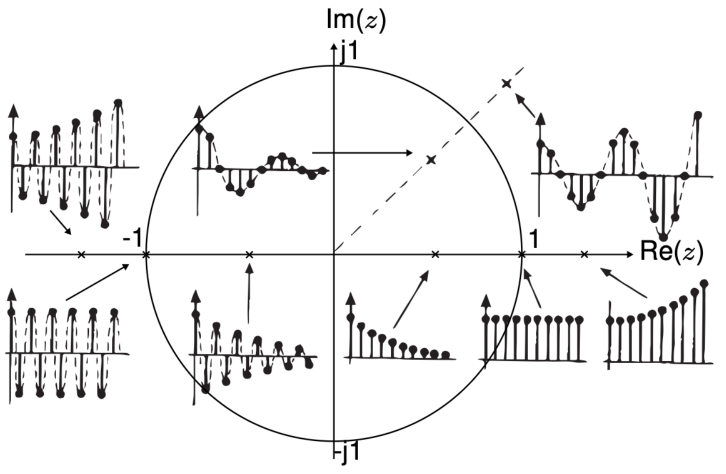
\includegraphics[width=0.5\textwidth]{Images/Impluse-response.png}
\end{center}
\subsection{Stability}
\textbf{Stable system:} A system is stable if its impulse response $h(n)$ goes to zero when $n$ goes to infinity.
$$|h(n)|\to 0 \quad\text{when }n\to \infty$$
If all poles of the transfer function $H(z)$ are inside the unit circle.
$$|p_i|\leq 1\quad\text{for }i=1,2,\dots,N$$

\textbf{Marginally stable system:} A system is marginally stable if its impulse response $h(n)$ approaches a constant value different from zero or oscillates with constant amplitude and frequency as it approaches infinity.

If one pole of the transfer function $H(z)$ are on the unit circle and the rest are inside.
$$|p_i|\leq 1\quad\text{for }i=1,2,\dots,N$$
$$|p_j|= 1\quad\text{for }j\in\{1,2,\dots,N\}$$

\textbf{Unstable system:} A system is unstable if its impulse response $h(n)$ grows indefinitely as it approaches infinity.
$$|h(n)|\to \infty \quad\text{when }n\to \infty$$
If one pole of the transfer function $H(z)$ are outside the unit circle.
$$|p_j|> 1\quad\text{for }j\in\{1,2,\dots,N\}$$

\subsection{Frequency response analysis}
A frequency response analysis gives the response of a system at a sinusoidal input sequence.
$$y(n)=AM(\omega)\cos(\omega t+\varphi(\omega))$$
where
$$M(\omega)=|H(j\omega)| \qquad \qquad\varphi(\omega)=\angle H(j\omega)$$
$$H(j\omega)=H(z)|_{z=e^{j\omega}T}\qquad\qquad H(j\omega)=|H(\omega)|\angle\varphi(\omega)$$

\subsection{Examples}
\subsubsection{Example 1: Stability}
Is the following transfer function stable?
$$G(z)=\frac{(z+0.2)(z-0.2)}{(z+0.5)(z-1.1)}$$

\rule{\textwidth}{0.5pt}

Looking at the poles we see:
$$p_1=-0.5\qquad p_2=1.1$$
Since $|p_2|> 1$ the transfer function is not stable.
\subsubsection{Example 2: Stability}
Is the following transfer function stable?
$$G(z)=\frac{z+2}{(z-0.9)(z+0.2)}$$

\rule{\textwidth}{0.5pt}

Looking at the poles we see:
$$p_1=0.9\qquad p_2=-0.2$$
Since $|p_1|< 1$ and $|p_2|< 1$ the transfer function is stable.

\subsubsection{Example 3: Impluse Response}
Find the Impluse Response Sequence of the following discrete transfer function:
$$G(z)=\frac{Y(z)}{X(z)}=\frac{1}{1-0.75z^{-1}+0.125z^{-2}}$$

\rule{\textwidth}{0.5pt}

The input impluse $x(n)=\delta(n)$:
$$G(z)=\frac{Y(z)}{X(z)}=1\cdot\frac{z^2}{z^2-0.75z+0.125}$$
Factor:
$$G(z)=\frac{z^2}{(z-0.5)(z-0.25)}$$
$$G(z)=\frac{z}{z-0.5}\cdot\frac{z}{z-0.25}$$
Inverse z-transformation:
$$g(n)=\mathcal{Z}^{-1}\left\{\frac{z}{z-0.5}\right\}\cdot\mathcal{Z}^{-1}\left\{\frac{z}{z-0.25}\right\}$$
Using table lookup (ZT4):
$$a^n=\mathcal{Z}^{-1}\left\{\frac{z}{z-a}\right\}$$
$$g(n)=0.5^n\cdot 0.25^n$$

\subsubsection{Example 3: Frequency Response}
